\documentclass{article}
\usepackage[english]{babel}
\usepackage[a4paper,top=2cm,bottom=2cm,left=2cm,right=2cm,marginparwidth=1.75cm]{geometry}
\usepackage{amsmath}
\usepackage{graphicx}
\usepackage{subcaption} 
\usepackage[colorlinks=true, allcolors=blue]{hyperref}
\usepackage{float}
\usepackage{titling}
\setlength{\droptitle}{-5em} 

\title{\textbf{Machine Learning: Exercise 0}}
\author{\textit{Amélie Assmayr (12007770)} \and
        \textit{Konstantinos Damanakis (12106343)} \and
        \textit{Teresa Schuch (12007762)}}
\date{}

\begin{document}
\maketitle
\vspace{-45pt}

\section{Introduction}
\vspace{-8pt}
In this Exercise we have chosen two datasets: Laptop Prices and Road Traffic Accidents. The Laptop Prices dataset will be utilized to develop regression models for predicting laptop prices , while the Road Traffic Accidents dataset will be employed to classify the severity of accidents. We chose these datasets because they enable us to try various techniques as they differ in important aspects. The Laptop Prices dataset has 2275 instances, 15 features and no missing values. In contrast, the Road Traffic Accidents dataset contains 12316 instances, 32 features and missing values in 16 features, making the preprocessing more important and complex.

\vspace{-8pt}
\section{Dataset 1: Laptop Prices}
\vspace{-8pt}
The Laptop Price dataset contains information about various laptops and their price in euros. We chose this dataset because of its importance in real-life situations. Most people today rely on laptops for work, education and entertainment. Predicting these prices can provide retailers with crucial insights into expected revenues before official pricing is announced. Additionally, the variety of features in the dataset, including both categorical and numeric data makes it ideal for experimenting with feature engineering. \newline
The variables, their data types and the number of unique values for nominal and ordinal variables can be seen below.
\begin{table}[H]
    \parbox{.45\linewidth}{
        \begin{tabular}{l|r|c}
            \textbf{Variable} & \textbf{Datatype} & \textbf{Unique}\\\hline
            \textit{Company} & nominal & 19 \\
            \textit{Product} & nominal & 618 \\
            \textit{Type Name} & nominal & 6 \\
            \textit{Inches} & ratio quantity & / \\
            \textit{Screen Resolution} & ordinal & 40 \\
            \textit{CPU Company} & nominal & 3 \\
            \textit{CPU Type} & nominal & 106 \\
            \textit{CPU Frequency} (GHz) & ratio quantity & /
        \end{tabular}
}
    \hfill
    \parbox{.45\linewidth}{
        \begin{tabular}{l|r|c}
            \textbf{Variable} & \textbf{Datatype} & \textbf{Unique}\\\hline
            \textit{RAM (GB)} & ratio quantity & / \\
            \textit{Memory} & ordinal & 39 \\
            \textit{GPU Company} & nominal & 4 \\
            \textit{GPU Type} & nominal & 106 \\
            \textit{Operating} System & nominal & 9 \\
            \textit{Weight (kg)} & ratio quantity & / \\
            \textit{Price (Euro)} & ratio quantity & / \\
            & &
        \end{tabular}}      
\end{table}

\vspace{-8pt}
\subsection{Target attribute}
\vspace{-8pt}
\begin{figure}[H]
\centering
\includegraphics[width=0.7\linewidth]{Histogram_Price.png}
\caption{\label{fig:hist:price} Histogram of Laptop Prices}
\end{figure}
\vspace{-10pt}
The target variable is the price of the laptop. The prices range between 174€ and 6099€. The histogram in Figure \ref{fig:hist:price} illustrates the distribution of the prices, revealing that most laptops are priced between 400 and 800€. The mean price is 1135€ and the median price 989 €. There are a few outliers that cost over 4000€, but these outliers are valid values. 

\vspace{-8pt}
\subsection{Additional Attribute Insights}
\vspace{-6pt}
The screensize ranges from 10.10 to 18.40 inches, with a mean of 15.02 inches. The weight varies between 0.690 kg and 4.7 kg, with an average weight of 2.041 kg. The CPU frequency spans from 0.9 to 3.6 GHz, with a mean value of 2.5 GHz and RAM takes integer values between 2 and 64 GB, with a median value of 8 GB. The variable product may require preprocessing and summarizing due to its numerous unique values. \newline
Due to limited space not all variable plots could be displayed. In Figure \ref{fig:Laptop} the distribution of RAM and the Top 10 Companies can be seen as an example.
\begin{figure}[H]
  \centering
  \begin{subfigure}[b]{0.45\textwidth}
    \includegraphics[width=\textwidth]{Ram.png}
    \caption{Barplot of RAM}
    \label{fig:ram}
  \end{subfigure}
  \hfill
  \begin{subfigure}[b]{0.45\textwidth}
    \includegraphics[width=\textwidth]{Comp.png}
    \caption{Barplot of the Top 10 Companies}
    \label{fig:company}
  \end{subfigure}
  \caption{Plots from Laptop dataset}
\label{fig:Laptop}
\end{figure}


\vspace{-20pt}
\section{Dataset 2: Road Traffic Accidents}
\vspace{-8pt}
The second dataset includes instances of road traffic accidents recorded in the years 2017 to 2020 in Addis Ababa in Ethiopia. This dataset contains information regarding severity of the accident, the number and the characteristics of the involved vehicles and  people, area etc.We chose this dataset because it addresses a critical public safety issue. A study of this data could help predict the severity of the accidents which can help identify causes and factors contributing to road safety. \newline
Missing data can be observed in 16 of the 32 features. Overall there are s 20.057 missing values. In the following table all attributes, their datatype(r=ratio quantity, o=ordinal, n=nominal), the number of unique elements for categorical variables and the number of missing values can be seen :
\begin{table}[H]
    \parbox{.5\linewidth}{
        \begin{tabular}{l|r|c|c}
            \textbf{Variable} & \textbf{Type} & \textbf{Unique} & \textbf{Missing}\\\hline
            \textit{Time} & r & / & / \\
            \textit{Day of Week} & n & 7 & /\\
            \textit{Age of Driver} & o & / & /\\
            \textit{Sex of Driver} & n & 3 &/ \\
            \textit{Educational Level} & n & 7 & 741\\
            \textit{Vehicle-Driver Relation} & n & 4 & 579 \\
            \textit{Driving Experience} & o & / & 829\\
            \textit{Vehicle Type} & n & 17 & 950\\
            \textit{Vehicle Owner} & n & 4 & 482\\
            \textit{Vehicle Service Year} & r & / & 3928\\
            \textit{Defect of Vehicle} & n & 3 & 4427\\
            \textit{Accident Area} & n & 14 & 239\\
            \textit{Lanes or Medians} & n & 7 & 385\\
            \textit{Road Alignment} & n & 9 & 142\\
            \textit{Junction Type} & n & 8 & 887\\
            \textit{Road Surface Type} & n  & 4 & 172
        \end{tabular}
}
    \hfill
    \parbox{.5\linewidth}{
        \begin{tabular}{l|r|c|c}
            \textbf{Variable} & \textbf{Type} & \textbf{Unique} & \textbf{Missing}\\\hline
            \textit{Road Surface Condition} & n & 4 & 172\\
            \textit{Light Condition} & n & 4 & /\\
            \textit{Weather Condition} & n & 9 &/\\
            \textit{Collision Type} & n & 10  & 155\\
            \textit{Number of Vehicles} & r & / &/\\
            \textit{Number of Casualty} & r & / &/\\
            \textit{Vehicle Movement} & n & 13 & 308\\
            \textit{Casualty Class} & n & 4 &/ \\
            \textit{Sex of Casualty} & n & 3 & / \\
            \textit{Age of Casualty} & r & / & /\\
            \textit{Casualty Severity} & o & 4 & / \\
            \textit{Work of Casualty} & n & 7 & 3198\\
            \textit{Fitness of Casualty} & n & 5 & 2635 \\
            \textit{Pedestrian Movement} & n & 9 &/ \\
            \textit{Cause of Accident} & n & 20 & /\\
            \textit{Severity of Accident} & n & 3 & /
        \end{tabular}}
\end{table}

\vspace{-8pt}
\subsection{Target Attribute}
\vspace{-6pt}
The target variable is the severity of the accident. It is classified into three classes: Light Injury, Serious Injury or Fatal Injury. While the severity could be considered an ordinal variable, we will treat it as nominal, framing the task as a multiclass classification problem. The following plot shows the distribution of these classes. It can be seen that the classes are unevenly distributed. Most accidents fall under the "Slight Injury" category, followed by "Serious Injury" and only a few accidents are classified as "Fatal Injury." This imbalance is a critical factor to consider. Methods like bootstrapping might be helpful to employ. 

\begin{figure}[H]
\centering
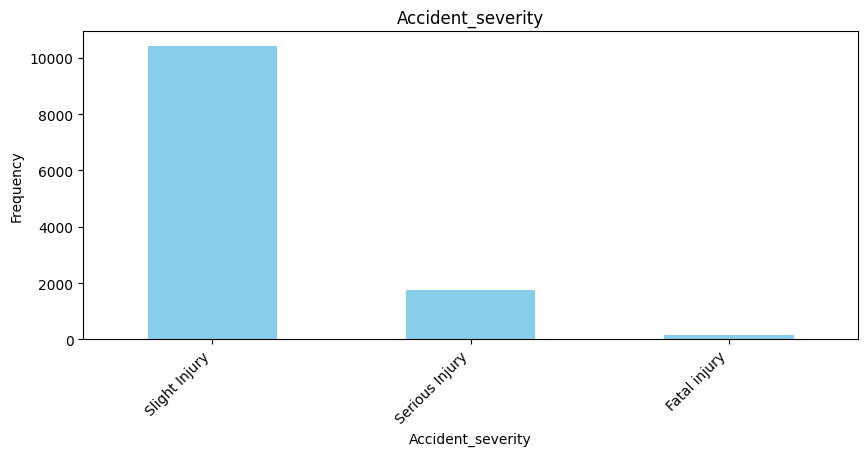
\includegraphics[width=0.7\linewidth]{Accident_severity.png}
\caption{\label{fig:hist:severity} Barplot of Accident Severity}
\end{figure}

\vspace{-20pt}
\subsection{additional attribute insights}
\vspace{-8pt}
Most of the numeric variables in the dataset are grouped into intervals, effectively converting them into ordinal data. Besides regular missing values, the dataset also has other entries like 'Unknown' or 'na' that should be handled during preprocessing. As an example the histogram of the time of the accident and the barplot of the age classses of the driver are shown below in Figure \ref{fig:Accident}:

\begin{figure}[H]
    \centering
    \begin{subfigure}[b]{0.45\textwidth}
        \centering
        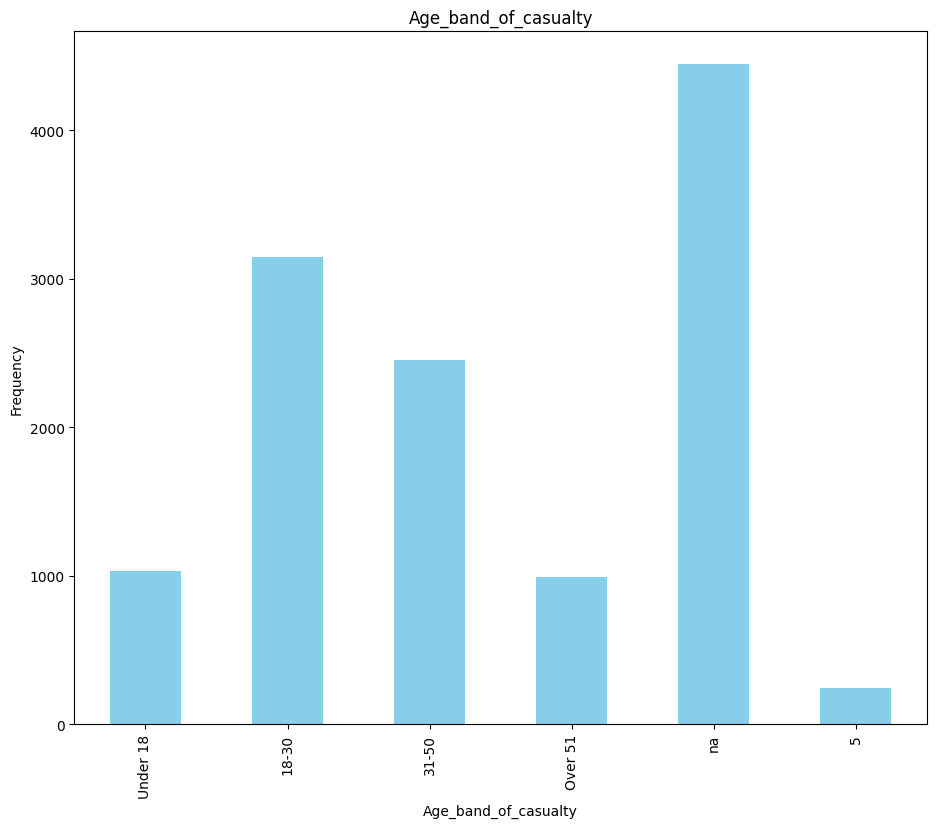
\includegraphics[width=1\linewidth]{Age_band_of_casualty.png}
        \caption{ Barplot of the age classes}
        \label{fig:bar:casuality}
    \end{subfigure}
    \hspace{0.05\textwidth}
    \begin{subfigure}[b]{0.45\textwidth}
        \centering
        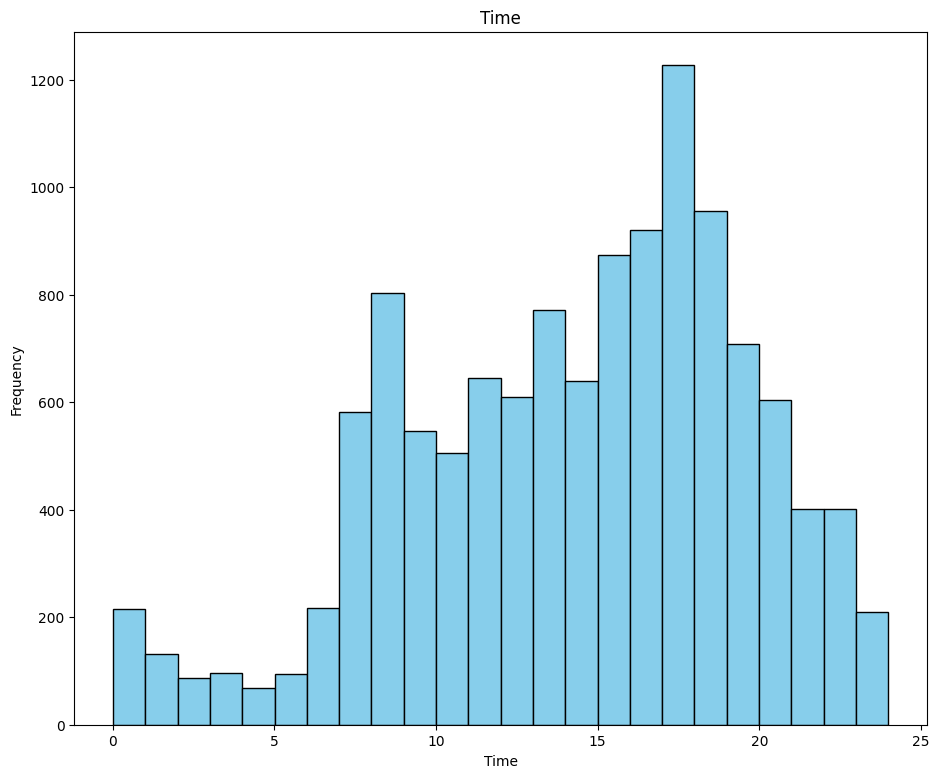
\includegraphics[width=1\linewidth]{Time.png}
        \caption{ Histogram of the Time}
        \label{fig:bar:time}
    \end{subfigure}
    \caption{Plots from Road Traffic Accident dataset}
    \label{fig:Accident}
\end{figure}

\end{document}